\chapter{Estado del arte}
\section{Blockchain}
\subsection{Definición}
Una blockchain \cite{blockchain-simple} es, en esencia, un libro de cuentas (o ledger) distribuido a lo largo de una red de nodos que la gestionan de forma no jerárquica, y en la que todos los nodos verifican las transacciones una a una antes de añadirlas a un bloque, que entonces se añade a la cadena y se descarga en cada nodo.
\begin{figure}[h]
\centerline{\includegraphics[scale=.25]{recursos/Cómo_funciona_Blockchain_Paso_a_paso.jpg}}
\caption{Funcionamiento de una blockchain.}
\label{blockchain-funcionamiento}
\end{figure}

Como bien indica su nombre, una blockchain es una cadena de bloques, en la que todos sus elementos principales (nodos, bloques y transacciones) están identificados por un hash. Los bloques están formados por una o mas transacciones, y las transacciones se ordenan mediante hashes creados a partir del hash de la transacción anterior y la siguiente, creando así una estructura que no se puede modificar sin cambiar todos los hashes de la cadena.
\subsection{Tipos}
Una red blockchain puede ser de 4 tipos distintos, implementados por tecnologías distintas, y que se adaptan a distintos casos de uso u organizaciones:
\begin{figure}[h]
\centerline{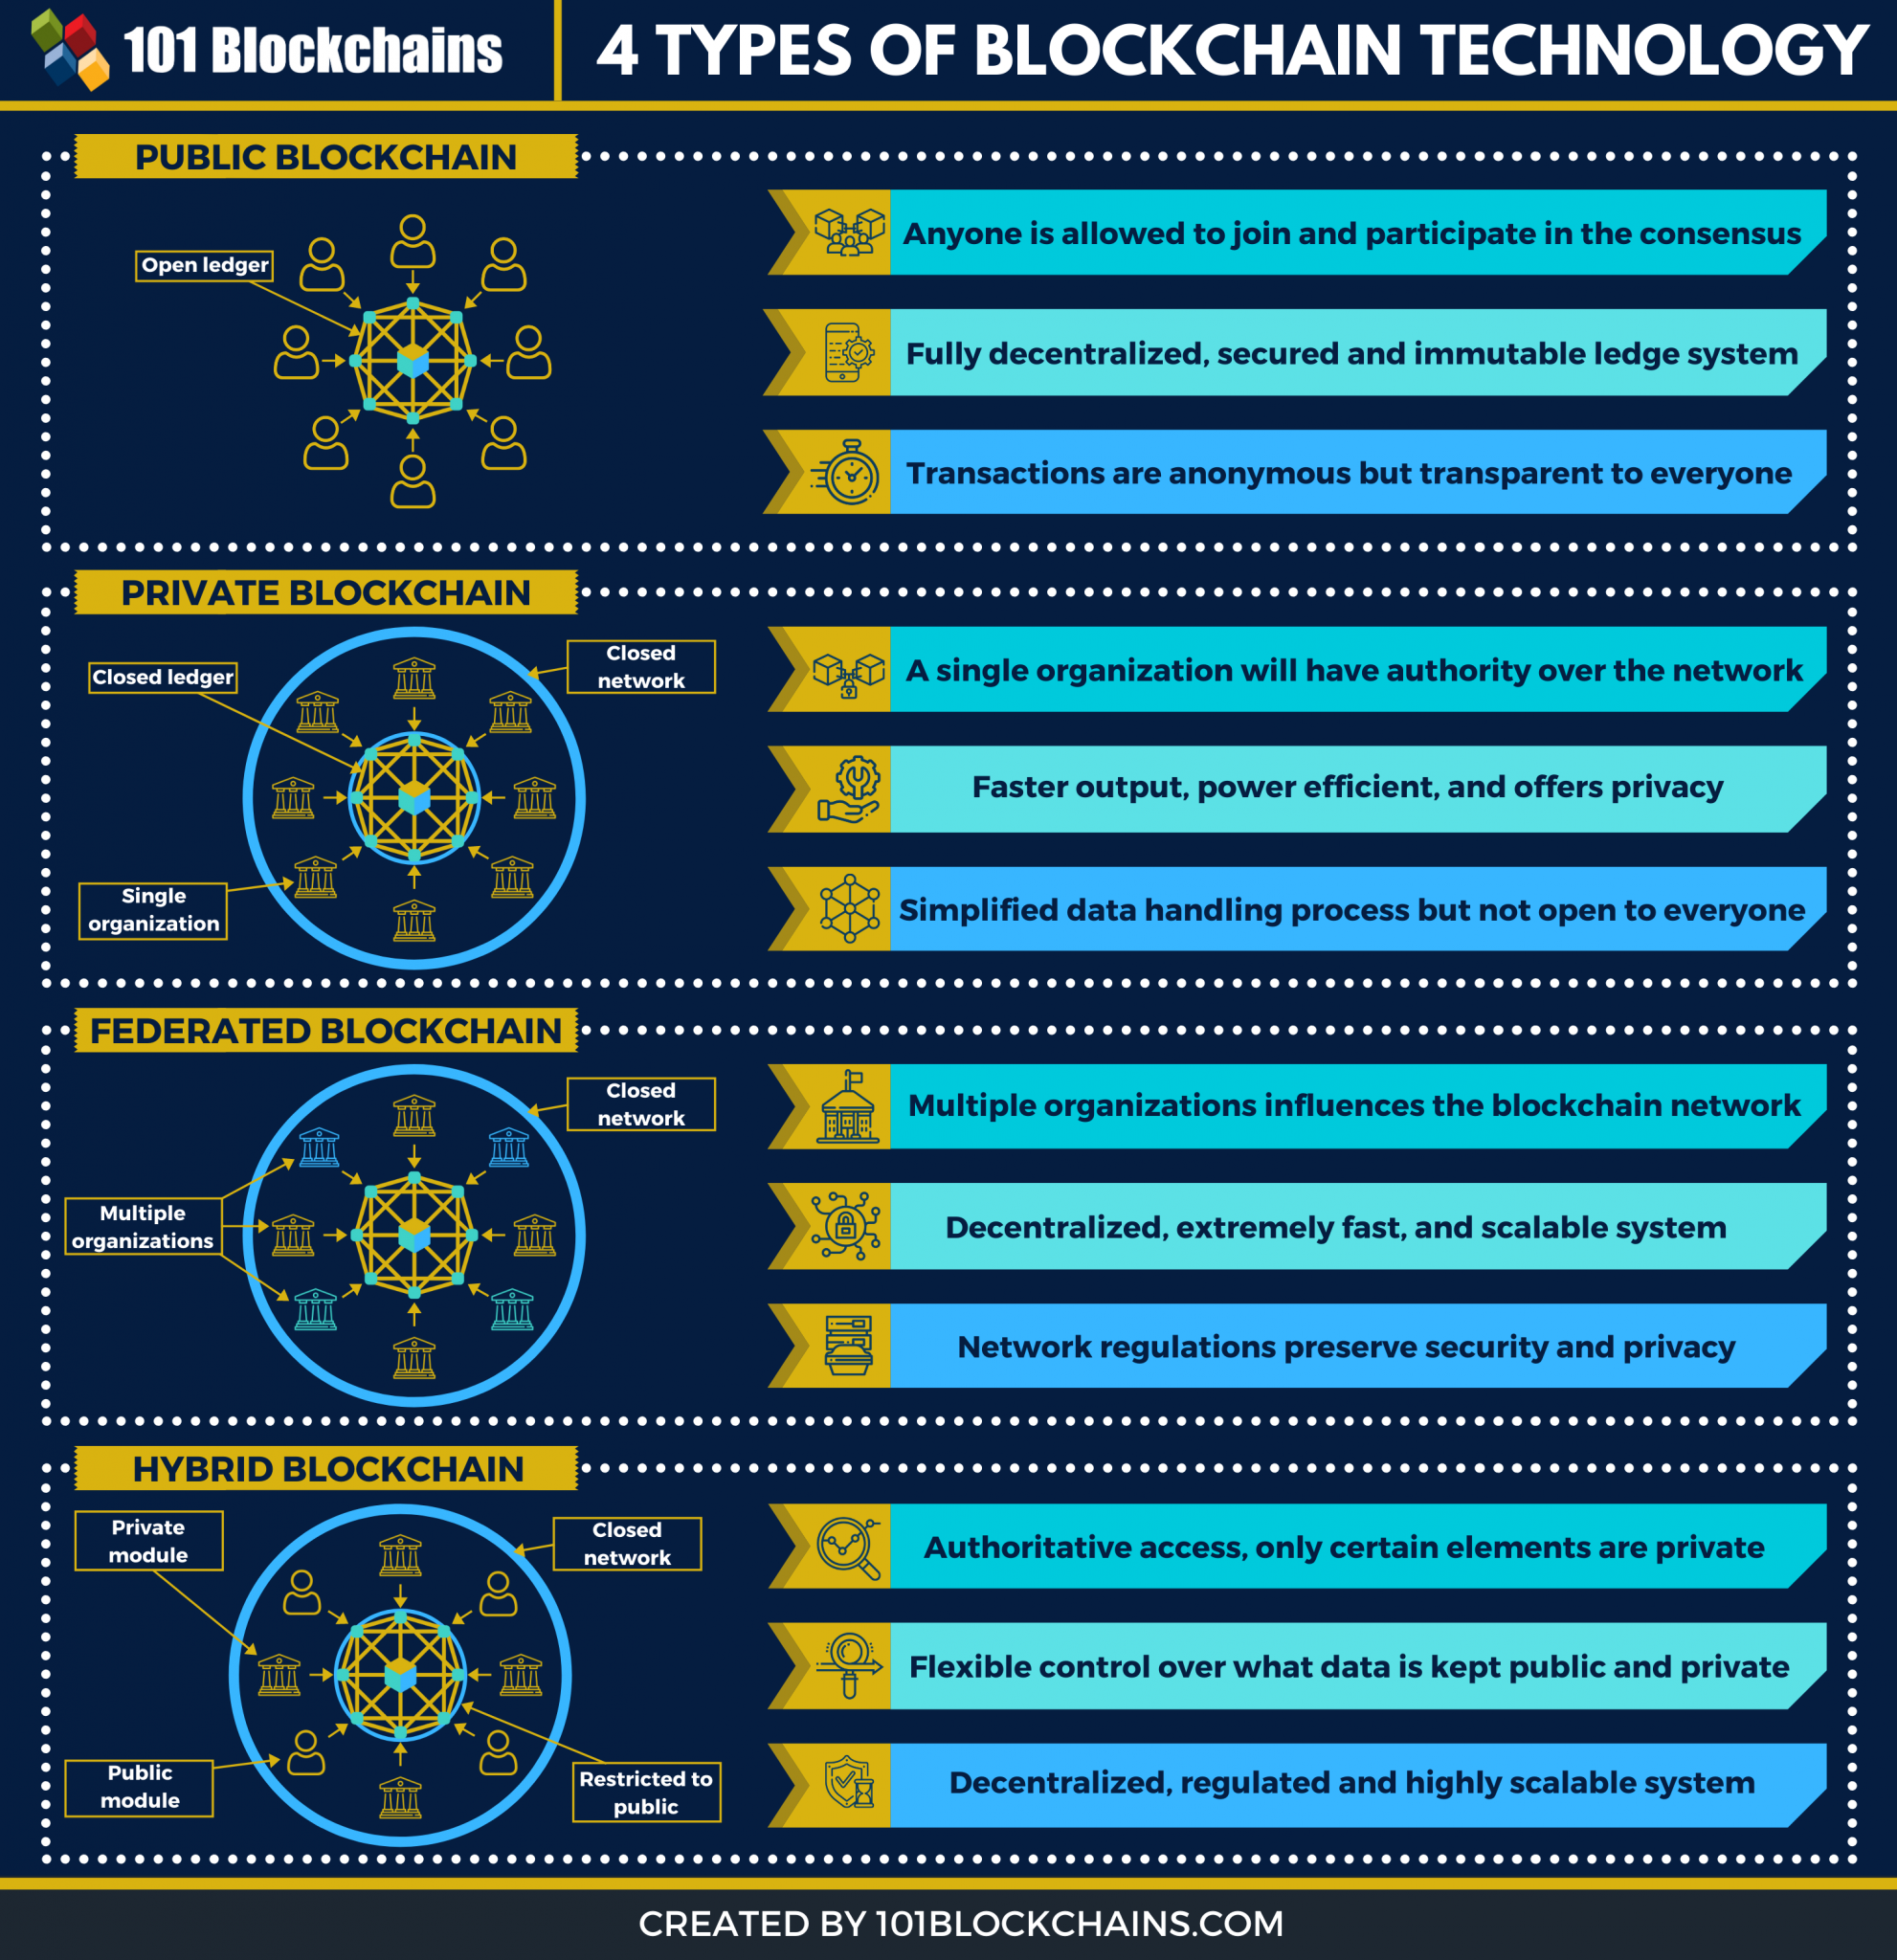
\includegraphics[scale=.2]{recursos/Types-of-Blockchain-Technology-1982x2048.png}}
\caption{Tipos de redes blockchain.}
\label{tipos-BC}
\end{figure}

\begin{enumerate}
\item \textbf{Pública:} En este tipo de redes, no hay ningún sistema de permisos, y cualquier entidad puede acceder a la blockchain y llevar a cabo transacciones. Esto conlleva que la verificación sea muy lenta, debido a los algoritmos utilizados para validar cada transacción, como Proof of Work \cite{POW}. Un ejemplo son las redes Ethereum \cite{ethereum}.
\item \textbf{Privada:} Una red privada funciona normalmente en entornos cerrados, como en el dominio de una compañía, y siempre están gestionadas por una entidad, lo que fuerza cierto grado de centralización. Las redes privadas solo permiten el acceso a entidades selectas, lo que las convierte por defecto en redes permisionadas, de las que hablaremos mas adelante. Por lo demás, su funcionamiento es idéntico al de una red pública. Un ejemplo son las redes Hyperledger Fabric \cite{fabric}.
\item \textbf{Federada/Consorcio:} Las redes federadas tienen partes públicas y partes privadas, y están diseñadas con el objetivo de facilitar la colaboración de varias empresas o entidades en la misma red. A diferencia de las privadas, en las redes federadas el control se comparte entre varias organizaciones, por lo que son mas descentralizadas que las anteriormente mencionadas. Un ejemplo de este tipo de red es Marco Polo.
\item \textbf{Híbrida:} En este tipo de red, se intentan combinar las características de las redes públicas y privadas, con una arquitectura muy maleable, que se puede adaptar a todo tipo de circunstancias, sin dejar de lado aspectos importantes como la transparencia o la seguridad. El acceso sigue estando regulado, pero hay partes públicas y privadas, cosa que depende enteramente de la red en particular. Un ejemplo son las redes Dragonchain.
\end{enumerate}

Además de estos cuatro tipos, existe una característica extra que puede añadirse a estas redes, y es que pueden ser permisionadas o no. Una red permisionada utiliza sistemas de identificación con las entidades que quieren utilizarla, además de asignación de roles para restringir el acceso a ciertas partes de la red a usuarios mas privilegiados. Un ejemplo de red pública permisionada son las basadas en Corda.

\section{Alastria ID}
Alastria ID es el modelo de identidad planteado por el consorcio Alastria, y que se basa en tres pilares fundamentales, siguiendo los principios de la identidad soberana que vimos anteriormente.
\begin{figure}[H]
\centerline{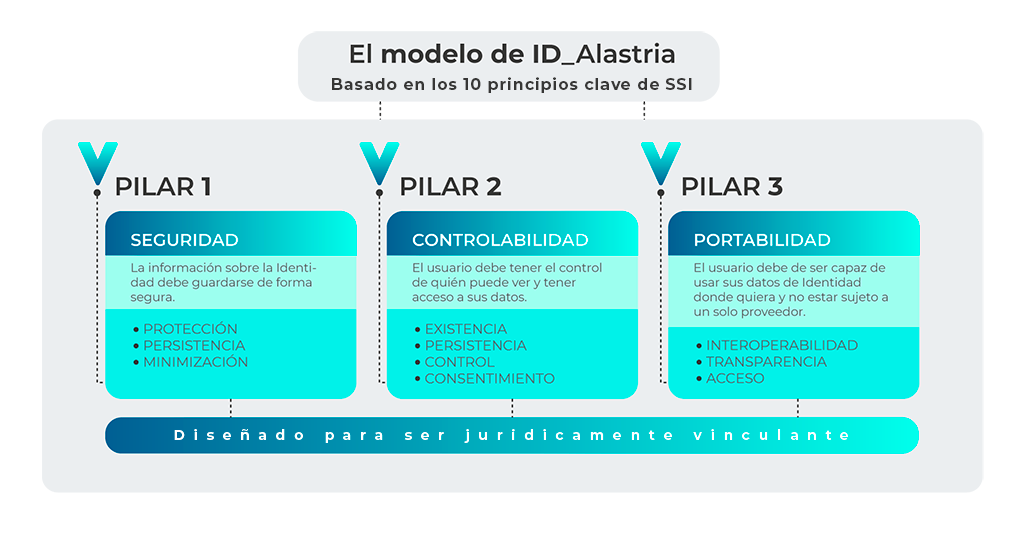
\includegraphics[scale=.5]{recursos/ID-Model-Esp-1.png}}
\caption{Pilares de Alastria ID.}
\label{pilares-alastriaid}
\end{figure}
\begin{enumerate}
    \item \textbf{Seguridad:} La información sobre la identidad se guarda en un \textit{wallet}, una aplicación móvil que aloja los datos en una zona altamente segura del dispositivo.
    \item \textbf{Controlabilidad:} El usuario controla sus datos por completo gracias a que se almacenan en su propio dispositivo, y gracias al uso de las credenciales y la capacidad para revocar su uso en cualquier momento.
    \item \textbf{Portabilidad:} Los datos del usuario siempre están con él gracias a que se guardan en el wallet. Además Alastria ID cuenta con capacidad para recuperar datos en caso de pérdida o robo.
\end{enumerate}
\subsection{Roles}
En el intercambio de credenciales y en todas las operaciones con Alastria ID, cada participante tiene un rol, ya sea una empresa, organización o individuo.
\begin{itemize}
    \item \textbf{Entity/Entidad:} Una entidad representa a una organización o empresa, pero no a un individuo.
    \item \textbf{Issuer/Emisor:} Entidad que tiene la posibilidad de crear credenciales y otorgarlas, ya sea a sujetos o a otras entidades. 
    \item \textbf{Service Provider/Proveedor de Servicios:} Entidad que proporciona servicios a sujetos o a otras entidades, utilizando opcionalmente credenciales. Son las encargadas de crear solicitudes de presentación y de recibir presentaciones con las credenciales requeridas para sus servicios.
    \item \textbf{Subject/Sujeto:} Persona física que se beneficia de las entidades, ya sea recibiendo credenciales de los emisores o servicios de los proveedores de servicio. Es propietario de un wallet de identidad, donde guarda sus credenciales y mediante el que recibe y envía solicitudes de presentación y presentaciones, respectivamente.
\end{itemize}
Cabe destacar que una entidad puede ser emisor y proveedor de servicio al mismo tiempo, e interactuar con otras entidades y recibir credenciales y servicios como si fuese un sujeto.
\subsection{DID}
DID significa \textit{Decentralized Identifier}, y puede referirse a cualquier tipo de sujeto (por ej.: personas, empresas, modelos de datos, entidades abstractas, etc...), están diseñados para ser completamente independientes de registros centralizados, y son capaces de demostrar que su propietario tiene el control sobre el elemento representado, sin necesidad de actores externos.

En Alastria ID, los DIDs se usan para representar a las entidades y a los sujetos, y tienen el siguiente formato \cite{did-credentials-presentations}:
\begin{verbatim}
did                     = "did:ala:" red ":" string-identificador
red                     = ("quor" / "fabr") ":" id-red
string-identificador    = depende de la red
\end{verbatim}
La definición de los componentes:
\begin{itemize}
    \item \textbf{ala:} Significa que este DID es de Alastria ID
    \item \textbf{red:} Especifica la tecnología que utiliza la red blockchain a la que pertenece el DID. Actualmente se utiliza ``quor'' para la red Quorum, pero próximamente se podrá utilizar ``fabr'' para la red Fabric.
    \item \textbf{id-red:} Representa la red blockchain específica, por ejemplo ``redt''.
    \item \textbf{string-identificador:} Depende de la red a la que pertenezca el DID. En la red disponible actual, que es la de Quorum, es la dirección Ethereum del "Proxy Contract" que representa al Alastria ID de la entidad. Su funcionamiento en la red Fabric se tratará en un apartado posterior.
\end{itemize}
\clearpage
\subsection{PSMHashes}
Tanto las credenciales como las presentaciones se representan e identifican mediante los llamados \acrshort{psmhash}. Un \acrshort{psmhash} es el hash de la suma del \acrshort{did} y la credencial o presentación. Cada credencial o presentación tiene dos \acrshort{psmhash}es, uno formado con el DID del emisor y otro con el DID del sujeto.
\begin{figure}[H]
\centerline{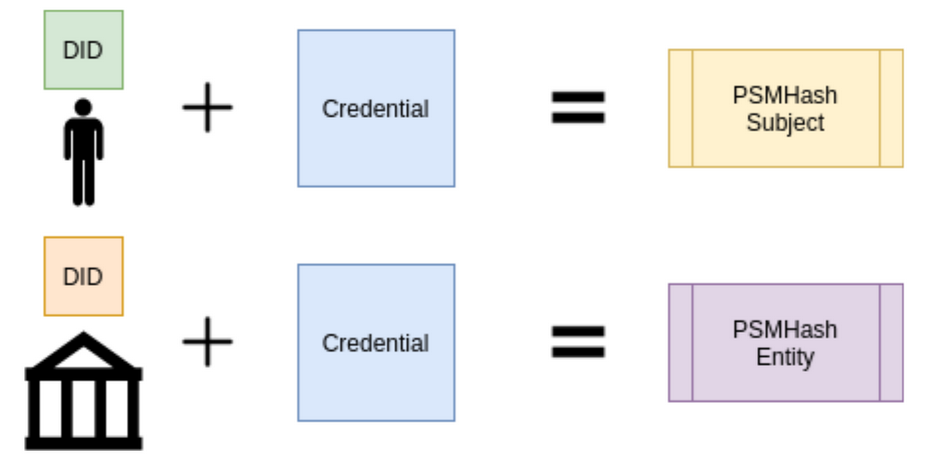
\includegraphics[scale=.7]{recursos/psmhashes.png}}
\caption{Estructura de los PSMHashes.}
\label{psmhashes}
\end{figure}
\subsection{Artefactos}
\subsubsection{Definición}
Los artefactos de Alastria son objetos \acrshort{jwt}, que tienen tres partes, \textit{header}, o cabecera, \textit{payload}, o cuerpo y \textit{signature}, o firma.
Cada una de estas partes se representa cifrada en Base64, y se unen mediante puntos (xxxx.yyyy.zzzz).
\subsubsection*{Cabecera}
Una cabecera esta formado por cuatro campos:
\begin{itemize}
    \item \textbf{alg:} Algoritmo utilizado para hashear el token
    \item \textbf{typ:} Tipo de token
    \item \textbf{kid:} Identificador de la clave pública utilizada. Opcional.
    \item \textbf{jwk:} Clave pública utilizada. Opcional.
\end{itemize}
Un ejemplo:
\begin{verbatim}
{
    "alg": "ES256K",
    "typ": "JWT",
    "kid": "did:ala:quor:redt:QmeeasCZ9jLbX...ueBJ7d7csxhb#keys-1",
    "jwk": "0x2e507af01167c98a6acc...83cf9779e4ea98d13df2833f3767"
}
\end{verbatim}
\subsubsection*{Cuerpo}
Depende del tipo de artefacto, en Alastria son \acrshort{at}, \acrshort{as} y \acrshort{aic}. También se incluyen las credenciales, solicitudes de presentación y presentaciones.
\subsubsection*{Firma}
La firma debe utilizar el algoritmo especificado en la cabecera, e incluye todo el \acrshort{jwt} a la hora de firmar.\\

En los siguientes apartados solo se describirá la parte del cuerpo de cada uno de los artefactos, puesto que tanto cabecera y firma utilizan siempre el mismo formato.
\subsubsection{JWTs de Alastria}
Hay tres objetos principales \cite{alastria-artifacts} utilizados en Alastria para la creación de identidades, la emisión de credenciales y la autenticación.
\subsubsection*{Alastria Token}
Se utiliza en cuatro flujos diferentes; la creación de identidades, la autenticación, la emisión de credenciales y en el envío de presentaciones.
Tiene seis campos obligatorios:
\begin{itemize}
    \item \textbf{iss:} DID del emisor del AT.
    \item \textbf{gwu:} URL del \textit{gateway} del que envía.
    \item \textbf{cbu:} URL de \textit{callback} a la que se debe responder.
    \item \textbf{ani:} Alastria Network ID. Identificador de la red de Alastria ID correspondiente.
    \item \textbf{iat:} Issued At. Tiempo de emisión del token.
    \item \textbf{exp:} Tiempo de expiración del token.
\end{itemize}
Tambien tiene cuatro campos opcionales:
\begin{itemize}
    \item \textbf{type:} Tipo de token (en este caso sería ``AlastriaToken'').
    \item \textbf{nbf:} NotBefore. Tiempo a partir del cual este token es válido.
    \item \textbf{jti:} Identificador único del JWT.
    \item \textbf{mfau:} \acrshort{mfau} URL. URL opcional para implementar autenticación multifactor.
\end{itemize}
Un ejemplo:
\begin{verbatim}
{
  "type": ["AlastriaToken","US12"]
  "nbf": 1587712704319,
  "gwu": "http://url/rpc",
  "cbu": "http://url/loginAID",
  "iss": "did:ala:quor:redT:3235c170482ff9ca250fb2a3b83468cb605f6a4c",
  "exp": 1587799104319,
  "ani": "redT",
  "iat": 1587712704319,
  "jti": "ze298y42sba",
  "mfau": "http://url/mfa_server"
}
\end{verbatim}
\subsubsection*{Alastria Session}
Su uso varía entre la autenticación de un usuario y la emisión de credenciales, y se distingue entre ellos añadiendo la historia de usuario correspondiente al campo \textit{type}.
Tiene cuatro campos obligatorios:
\begin{itemize}
    \item \textbf{@context:} URLs con la especificación del token, debe ser al menos\\ ``https://alastria.github.io/identity/artifacts/v1''.
    \item \textbf{type:} Tipo de token (en este caso sería ``AlastriaSession'').
    \item \textbf{iss:} DID del emisor del token. 
    \item \textbf{alastriaToken:} \acrshort{at} en formato \acrshort{jwt}. Es el AT al que este AS responde.
\end{itemize}
También puede tener cuatro campos opcionales mas; jti, iat, exp y nbf, que son los mismos que en el \acrshort{at} y en el \acrshort{aic}.
Un ejemplo de Alastria Session:
\begin{verbatim}
{
  "jti": "ze298y42sba"  
  "@context": ["https://alastria.github.io/identity/artifacts/v1"],
  "type": ["AlastriaSession","US211"]
  "iss": "did:ala:quor:redT:07dba616e17a45fca5cfc999a584180e45353aa9",
  "iat": 1587712763,
  "exp": 1563783392,
  "nbf": 1563783392,
  "alastriaToken": "eyJ0..4ea8",
}
\end{verbatim}
\subsubsection*{Alastria Identity Creation}
Es el objeto que envían los sujetos desde el \textit{wallet} para registrar un nuevo Alastria ID, completando así el ultimo paso de la creación de identidad.
Tiene cinco campos obligatorios:
\begin{itemize}
    \item \textbf{@context:} URLs con la especificación del token, debe ser al menos\\ ``https://alastria.github.io/identity/artifacts/v1''.
    \item \textbf{type:} Tipo de token (en este caso sería ``AlastriaIdentityCreation'').
    \item \textbf{createAlastriaTX:} Transacción en hexadecimal de creación de Alastria ID, firmada por el sujeto.
    \item \textbf{alastriaToken:} \acrshort{at} en formato \acrshort{jwt}. Es el \acrshort{at} original al que este \acrshort{aic} responde. Cabe destacar que no está firmado, ya que está dentro de un \acrshort{aic} firmado.
    \item \textbf{publicKey:} Clave pública del sujeto en hexadecimal. 
\end{itemize}
También puede tener cuatro campos opcionales mas; jti, iat, exp y nbf, que son los mismos que en el \acrshort{at} y en el \acrshort{as}.
Un ejemplo:
\begin{verbatim}
{
  "@context": ["https://alastria.github.io/identity/artifacts/v1"],
  "type": ["AlastriaIdentityCreation","US12"],
  "createAlastriaTX":"0xf9...",
  "alastriaToken":"ey...",
  "publicKey":"0x2e...",
  "jti": "ze298y42sba",
  "iat": 1587712763,
  "exp": 1563783392,
  "nbf": 1563783392
}
\end{verbatim}
\subsubsection{Intercambio de credenciales}
Los objetos dedicados al intercambio de credenciales \cite{did-credentials-presentations} siguen el mismo formato \acrshort{jwt} de los artefactos de Alastria, y comparten la misma cabecera, que tiene los siguientes campos obligatorios:
\begin{itemize}
    \item \textbf{typ:} Tipo del formato, siempre es ``JWT''.
    \item \textbf{alg:} Algoritmo utilizado en la firma del \acrshort{jwt}, siempre es ES256K.
\end{itemize}
También tiene otros dos campos opcionales:
\begin{itemize}
    \item \textbf{kid:} Identificador de la clave pública usada para firmar el \acrshort{jwt}. En Alastria es el \acrshort{did} de la clave pública seguido por ``\#keys-1''.
    \item \textbf{jwk:} Clave pública usada para firmar el \acrshort{jwt}.
\end{itemize}
Un ejemplo:
\begin{verbatim}
{
    "alg": "ES256K",
    "typ": "JWT",
    "kid": "did:ala:quor:redt:3eabc53a851fc5...1cc4b2b5d1#keys-1",
    "jwk": "0x2e507af01167c98a6accc0c...ea98d13df2833f3767"
}
\end{verbatim}
El apartado de firma de estos \acrshort{jwt}s es siempre el mismo, expuesto en una sección anterior.
En los siguientes apartados se describirá la parte del cuerpo de los \acrshort{jwt}s de intercambio de credenciales. Todos los campos referentes a tiempo están en formato ``NumericDate'' de \acrshort{json}.
\subsubsection*{Credencial}
Las credenciales contienen datos sobre un sujeto o entidad, son otorgadas por un emisor y se entregan a los proveedores de servicio mediante presentaciones. 
Tienen seis campos simples y uno complejo, que contiene tres campos como mínimo:
\begin{itemize}
    \item \textbf{jti:} Identificador único de la credencial. Opcional.
    \item \textbf{iss:} \acrshort{did} de la entidad emisora de la credencial. Obligatorio.
    \item \textbf{sub:} \acrshort{did} del sujeto al que se le ha emitido la credencial. Opcional.
    \item \textbf{iat:} Tiempo de emisión de la credencial. Obligatorio.
    \item \textbf{exp:} Tiempo de expiración de la credencial. Opcional.
    \item \textbf{nbf:} Tiempo a partir del cual esta credencial es válida. Opcional.
    \item \textbf{vc:} \textit{Verifiable Credential}. Es el objeto que tiene la información en si de la credencial.
    \begin{itemize}
        \item \textbf{@context:} Un array de URLs con información sobre la definición de la credencial. Como mínimo debe contener \\
        ``https://alastria.github.io/identity/credentials/v1'' y \\``https://www.w3.org/2018/credentials/v1''.
        \item \textbf{type:} Un array con los tipos de credencial. Como mínimo debe contener ``VerifiableCredential'' y ``AlastriaVerifiableCredential''.
        \item \textbf{levelOfAssurance:} Es el nivel de confianza en la credencial. Está basado en los niveles de confianza de \acrshort{eidas}. Sus valores posibles son ``Self'', ``Low'', ``Substantial'' y ``High''. Se suele encontrar dentro de un campo llamado ``credentialSubject'', que contiene los datos que representa la credencial. Opcional.
    \end{itemize}
\end{itemize}
Un ejemplo:
\begin{verbatim}
{
  "jti": "https://www.oneweb.com/alastria/credentials/3732",
  "iss": "did:alastria:quorum:redt:c5039eae214608f...aeea381ccb5d1",
  "sub": "did:alastria:quorum:redt:3eabc53a851fc50...acf8cc4b2b5d1",
  "iat": 1525465044,
  "exp": 1530735444,
  "nbf": 1525465044,
  "vc": {
    "@context": [
      "https://www.w3.org/2018/credentials/v1",
      "https://alastria.github.io/identity/credentials/v1",
      "https://universities.io/examples/v1"
    ],
    "type": ["VerifiableCredential","AlastriaVerifiableCredential", 
            "UniversityDegreeCredential"],
    "credentialSubject": {
      "levelOfAssurance": 0,
      "degree": {
        "type": "BachelorDegree",
        "name": "Bachelor of Science and Arts"
      }
    }
  }
}
\end{verbatim}
\subsubsection*{Presentation/Presentación}
Las presentaciones contienen una o más credenciales, y son el medio por el que los proveedores de servicio reciben las credenciales necesarias de entidades o sujetos. Son la respuesta a las solicitudes de presentación.
Tienen siete campos simples y uno complejo, que contiene cinco campos mas:
\begin{itemize}
    \item \textbf{jti:} Identificador único de la presentation. Opcional.
    \item \textbf{iss:} \acrshort{did} del sujeto o entidad que ha creado la presentation. Obligatorio.
    \item \textbf{aud:} \acrshort{did} de la entidad a la que va destinada la presentation. Obligatorio.
    \item \textbf{iat:} Tiempo de creación de la presentación. Obligatorio.
    \item \textbf{exp:} Tiempo de expiración de la presentación. Opcional.
    \item \textbf{nbf:} Tiempo a partir del cual la presentación es válida. Opcional.
    \item \textbf{jtipr:} Identificador único de la solicitud de presentación asociada a la presentación. Opcional.
    \item \textbf{vp:} \textit{Verifiable Presentation}. Es el objeto que contiene la información de la presentación en si. Contiene cinco campos obligatorios.
    \begin{itemize}
        \item \textbf{@context:} Un array de URLs con información sobre la definición de la credencial. Como mínimo debe contener\\
        ``https://alastria.github.io/identity/credentials/v1'' y \\
        ``https://www.w3.org/2018/credentials/v1''.
        \item \textbf{type:} Un array con los tipos de presentación. Como mínimo debe contener ``VerifiablePresentation'' y ``AlastriaVerifiablePresentation''.
        \item \textbf{procHash:} Es el hash de un documento que describe el propósito de las credenciales que se envían. 
        \item \textbf{procUrl:} Es la URL donde se aloja un documento que describe el propósito de las credenciales que se envían. 
        \item \textbf{verifiableCredential:} Es un array de credenciales requeridas en formato \acrshort{jwt}.
    \end{itemize}
\end{itemize}
Un ejemplo:
\begin{verbatim}
{
  "jti": "https://www.empresa.com/alastria/credentials/3732",
  "iss": "did:alastria:quorum:redt:3eabc53...924a381cc4b2b5d1",
  "aud": "did:alastria:quorum:redt:3eabc53...924a381cc4b2b5d1",
  "iat": 1525465044,
  "exp": 1530735444,
  "nbf": 1525465044,
  "jtipr": "metrovacesa/alastria/presentationrequest/7864",
  "vp": {
    "@context": [
      "https://www.w3.org/2018/credentials/v1",
      "https://alastria.github.io/identity/credentials/v1",
    ],
    "type": ["VerifiablePresentation", "AlastriaVerifiablePresentation"],
    "procHash": "H398sjHd...kldjUYn475n",
    "procUrl": "https://www.empresa.com/alastria/businessprocess/4583",
    "verifiableCredential": [{ ... }]
  }
}
\end{verbatim}
\subsubsection*{Presentation Request/Solicitud de presentación}
Las solicitudes de presentación son el método que tienen los proveedores de servicio de solicitar las credenciales necesarias a los sujetos o entidades, con el fin de otorgar un servicio.
Tienen cinco campos simples y uno complejo, que a su vez contiene seis campos:
\begin{itemize}
    \item \textbf{jti:} Identificador único de la solicitud de presentación. Opcional.
    \item \textbf{cbu:} URL de \textit{callback} del proveedor de servicio. Obligatorio.
    \item \textbf{iss:} \acrshort{did} del proveedor de servicio que ha creado la solicitud de presentación. Obligatorio.
    \item \textbf{iat:} Tiempo de creación de la solicitud de presentación. Obligatorio.
    \item \textbf{exp:} Tiempo de expiración de la solicitud de presentación. Opcional.
    \item \textbf{pr:} Objeto que contiene los datos de la solicitud de presentación. Tiene cinco campos simples y uno complejo, que a su vez contiene cuatro campos:
    \begin{itemize}
        \item \textbf{@context:} Un array de URLs con información sobre la definición de la solicitud de presentación. Como mínimo debe contener\\
        ``https://alastria.github.io/identity/credentials/v1'' y \\
        ``https://www.w3.org/2018/credentials/v1''. Obligatorio.
        \item \textbf{type:} Un array con los tipos de solicitud de presentación. Como mínimo debe contener ``VerifiablePresentationRequest'' y\\ ``AlastriaVerifiablePresentationRequest". Obligatorio.
        \item \textbf{procHash:} Es el hash de un documento que describe el propósito de las credenciales que se solicitan. Obligatorio.
        \item \textbf{procUrl:} Es la URL donde se aloja un documento que describe el propósito de las credenciales que se solicitan. Obligatorio. 
        \item \textbf{procDesc:} Descripción del propósito de las credenciales que se solicitan. Opcional.
        \item \textbf{data:} Es un array en el que cada objeto representa una credencial solicitada. Tiene tres campos obligatorios y uno opcional:
        \begin{itemize}
            \item \textbf{@context:} Un array de URLs con información sobre la credencial. Obligatorio.
            \item \textbf{levelOfAssurance:} Es el nivel de confianza mínimo que se requiere de la credencial. Está basado en los niveles de confianza de \acrshort{eidas}. Sus valores posibles son ``Self'', ``Low'', ``Substantial'' y ``High''. Opcional.
            \item \textbf{required:} Es un booleano que especifica si la credencial es obligatoria o no. Obligatorio.
            \item \textbf{field\_name:} Nombre de la credencial requerida. Obligatorio.
        \end{itemize}
    \end{itemize}
\end{itemize}
Un ejemplo:
\begin{verbatim}
{
  "jti": "metrovacesa/alastria/presentationrequest/7864",
  "iss": "did:alastria:quorum:testnet1:3eabc53a851f...a381cc4b2b5d1",
  "iat": 1525465044,
  "exp": 1530735444,
  "nbf": 1525465044,
  "cbu": "https://www.metrovacesa.com/alastria/presentation?jtipr=7864"

  "pr": {
    "@context": [
      "https://www.w3.org/2018/credentials/v1",
      "https://alastria.github.io/identity/credentials/v1"
    ],
    "type": ["VerifiablePresentationRequest", 
        "AlastriaVerifiablePresentationRequest"],
    "procHash": "H398sjHd...kldjUYn475n",
    "procUrl": "https://www.ejemplo.com/alastria/businessprocess/4583",
    "procDesc": "Descripción corta del propósito de la PR",
    "data": [
      {
        "@context": ["https://alastria.github.io/identity/covid/v1"],
        "levelOfAssurance": 3,
        "required": true,
        "field_name": "covid_test",
      },
      {
        "@context": ["https://alastria.github.io/identity/examples/v1"],
        "levelOfAssurance": 2,
        "required": true,
        "field_name": "phone_number",
      }
    ]
  }
}
\end{verbatim}

\clearpage
\section{Hyperledger Fabric}
Hyperledger Fabric es una plataforma \acrshort{dlt} open source creada por Linux Foundation, y diseñada con el uso empresarial en mente, gracias a una arquitectura altamente modular y configurable, y que soporta smart contracts codificados en lenguajes de programación generales, como Java, Go o Node.js.
Las redes de Hyperledger Fabric son privadas permisionadas, lo que significa que los miembros requieren de autenticación para hacer uso de ellas, y lo que también implica que no hay necesidad de algoritmos de consenso pesados como \acrshort{pow} \cite{fabric-simple}.
En los siguientes apartados se describirán los componentes principales del modelo de Hyperledger Fabric.
\subsection{Nodos}
Una red Fabric está compuesta principalmente por uno o más nodos, que pueden ser de dos tipos, peers u orderers.
\subsubsection{Peers}
Los \textit{peers} son el elemento mas importante de una red Fabric, puesto que tanto los \textit{ledgers} como los \textit{chaincodes} se despliegan en ellos. Cada \textit{peer} puede contener tantas instancias de distintos \textit{ledgers} como se desee, así como cualquier cantidad de \textit{chaincodes} que accedan a ellos.
\begin{figure}[H]
\centerline{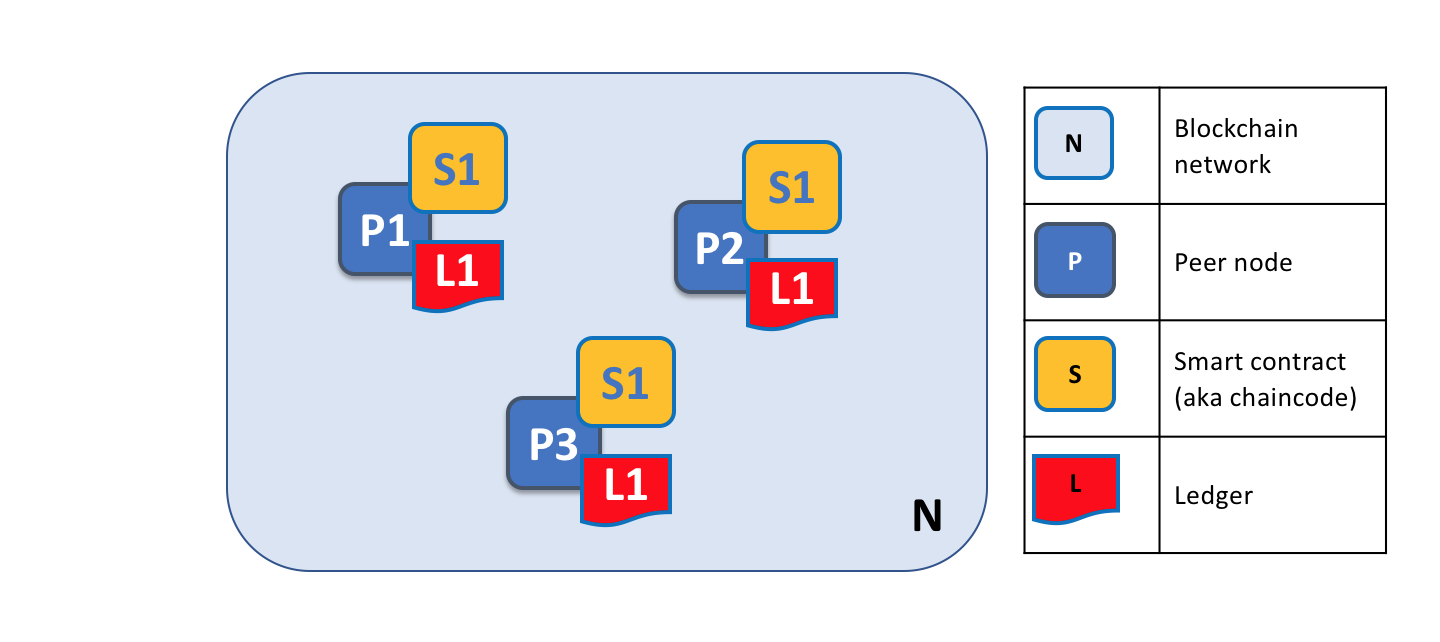
\includegraphics[scale=0.4]{recursos/peers.png}}
\caption{Red Fabric básica.}
\label{peers-network}
\end{figure}
Los \textit{peers} también exponen varias APIs para que aplicaciones externas puedan interactuar con la blockchain. Esto se hace mediante el uso de transacciones, y aquí es donde entran en juego los nodos \textit{orderer}, que se describirán en el siguiente apartado.
En la figura anterior, se puede observar que todos los nodos tienen instancias del mismo \textit{ledger} (L1), con sus correspondientes \textit{chaincodes} (S1). Esto es debido a que todos los nodos deben estar sincronizados para que sea posible una implementación descentralizada.
\begin{figure}[h]
\centerline{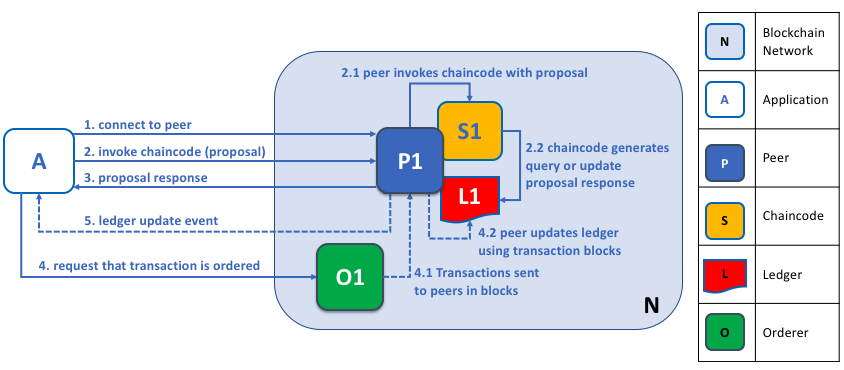
\includegraphics[scale=0.6]{recursos/peers-aplicacion.png}}
\caption{Interacción de una aplicación externa con la red.}
\label{peers-application}
\end{figure}
\clearpage
\subsubsection{Orderers}
Los nodos \textit{orderer} se encargan de ordenar las transacciones y de crear un bloque con ellas, para después enviarlo de vuelta a los \textit{peers} y que los \textit{ledgers} de todos ellos se mantengan sincronizados. Los \textit{orderers} son necesarios en redes con mas de un \textit{peer}, ya que, al generarse varias transacciones es necesario saber su orden para mantener las blockchains coordinadas.
\begin{figure}[H]
\centerline{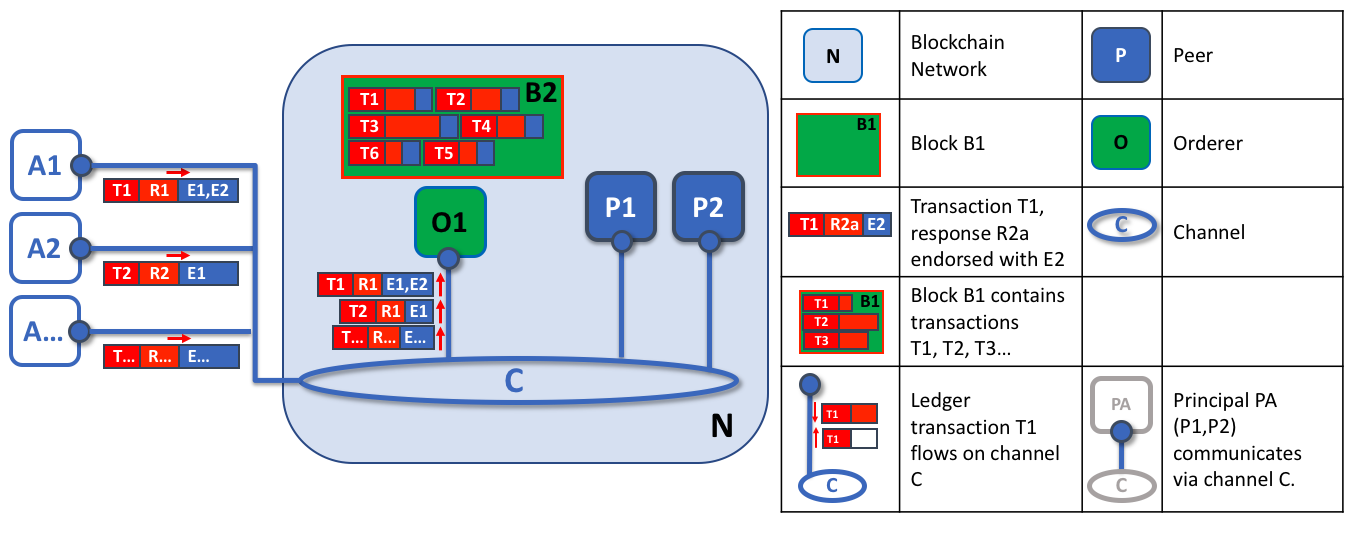
\includegraphics[scale=0.4]{recursos/orderers.png}}
\caption{Creación de bloques por parte del orderer.}
\label{orderers}
\end{figure}
En el diagrama anterior, se puede observar como las transacciones y sus respuestas ya validadas por los peers (T1, R1, validadas por E1 y E2) salen de las aplicaciones y van al \textit{orderer} (O1), que las ordena y las introduce en un bloque (B2). Este bloque se envía a todos los \textit{peers} para que actualicen el estado de sus \textit{ledgers} con la información de las transacciones.
Nótese que todos los elementos están conectados en el diagrama a un \textit{channel}, o \textit{channel}, que se describirá en el siguiente apartado.
\clearpage
\subsection{Channels/Canales}
Los \textit{channels}, o canales, son un mecanismo que se utiliza para que los componentes de una red Fabric puedan interactuar de forma privada entre ellos. Un peer puede formar parte de varios \textit{channels}, y cada \textit{channel} tiene sus propias reglas y configuración de acceso. Un \textit{channel} solo puede tener un ledger.
\begin{figure}[H]
\centerline{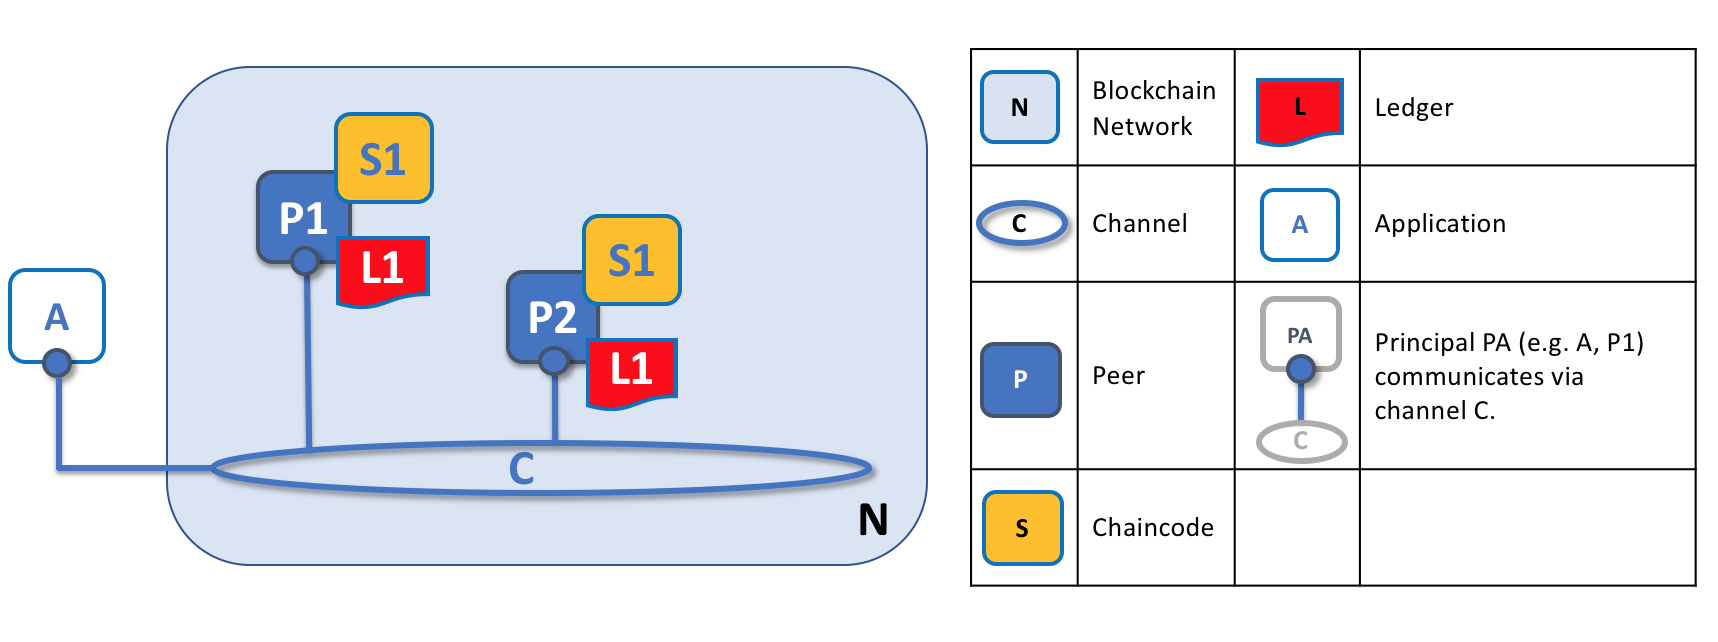
\includegraphics[scale=0.3]{recursos/canales.png}}
\caption{Red simple con un channel y dos peers.}
\label{canales}
\end{figure}
\subsection{Ledger}
En Fabric, un \textit{ledger} contiene la información sobre los objetos, y está compuesto de dos partes, la blockchain y el \textit{world state} (o \textit{state database}).
\begin{figure}[H]
\centerline{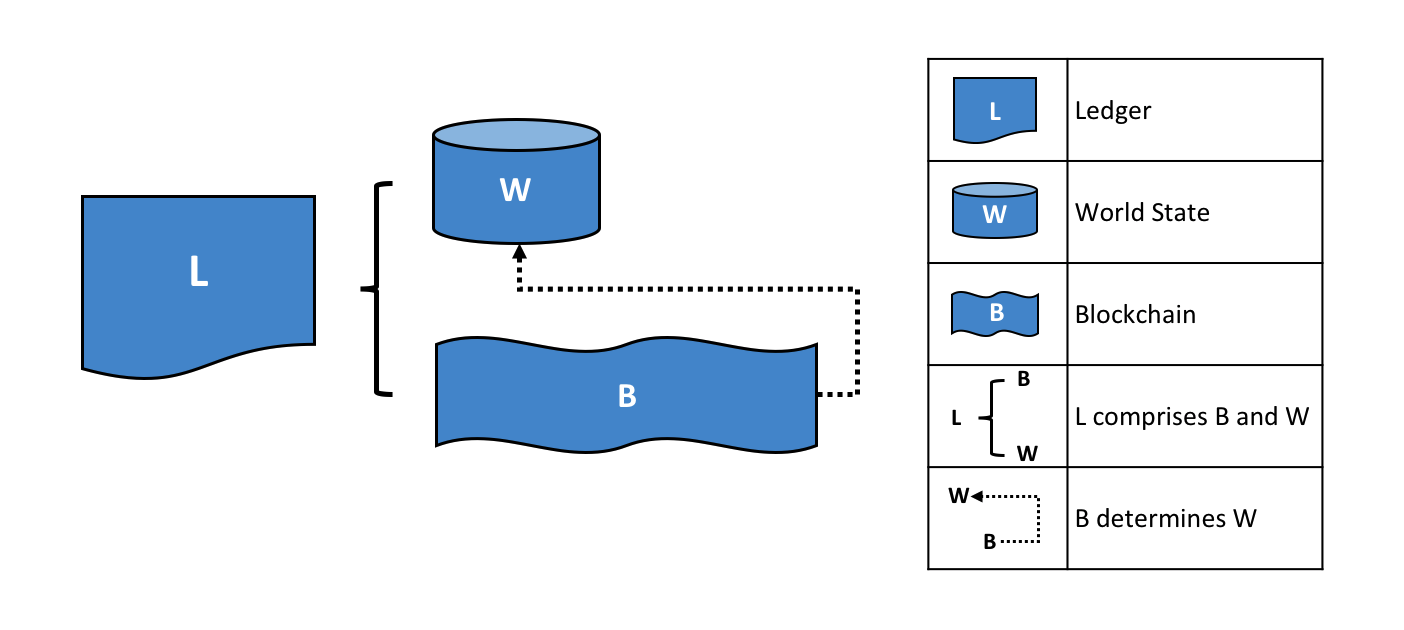
\includegraphics[scale=0.35]{recursos/ledger-partes.png}}
\caption{Un ledger y sus partes.}
\label{ledger}
\end{figure}
\subsubsection{World State/State Database}
El \textit{world state} o \textit{state database} guarda el valor de los objetos en formato clave-valor, además de controlar la versión de cada objeto individualmente.
\begin{figure}[H]
\centerline{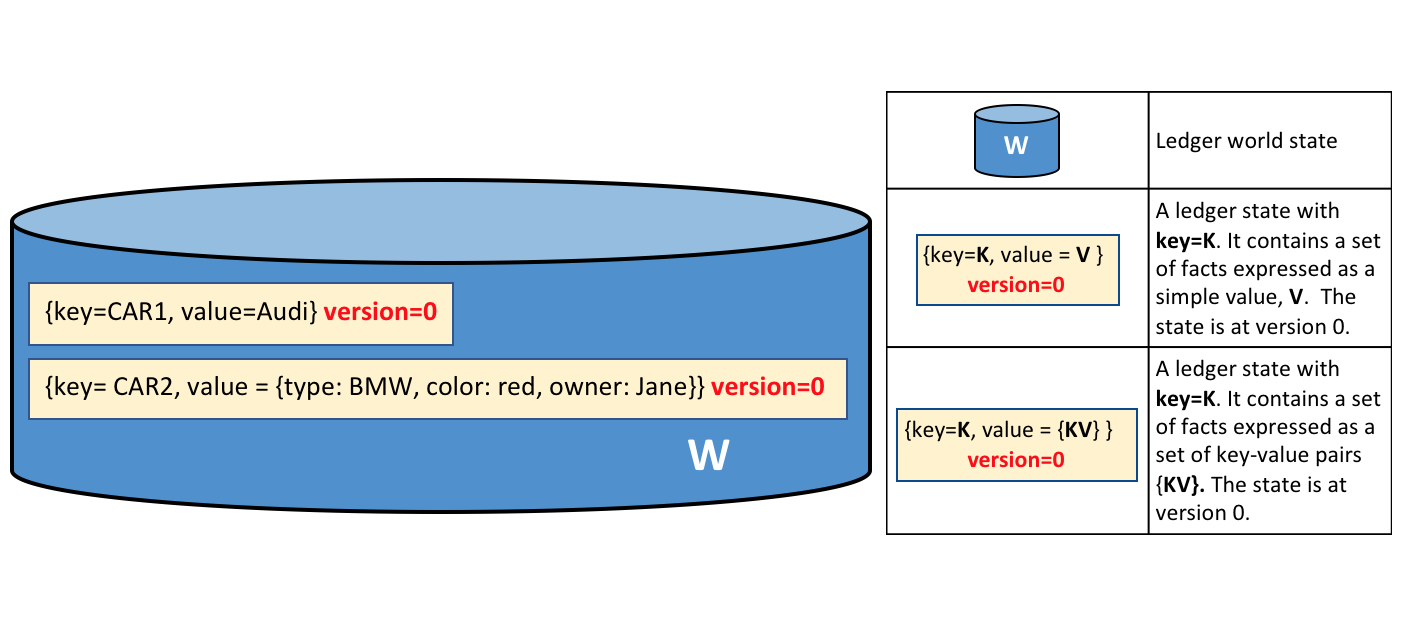
\includegraphics[scale=0.3]{recursos/world-state.png}}
\caption{Componentes de un world state típico.}
\label{world-state}
\end{figure}
En el diagrama se puede observar que los valores de los objetos pueden ser tanto simples como complejos.
El \textit{world state} es en realidad una base de datos, con todas las ventajas que eso conlleva. Hay distintos tipos de bases de datos disponibles, con diferentes características para diferentes proyectos.\\
La funcionalidad principal del \textit{world state} es almacenar todos los cambios en los estados del mundo, realizados por las transacciones, para que el acceso a estos sea lo mas cómodo y eficiente posible. Esto significa que el \textit{world state} es un reflejo de la blockchain, y puede regenerarse a partir de ella en cualquier momento.
\clearpage
\subsubsection{Blockchain}
La parte blockchain del \textit{ledger} es un registro histórico de todos los estados del \textit{ledger}, y está estructurada como una cadena de bloques, donde cada bloque contiene una o mas transacciones ordenadas, que contienen cambios sobre el \textit{world state}.\\
La blockchain esta implementada mediante un archivo, a diferencia del \textit{world state}.
\begin{figure}[H]
\centerline{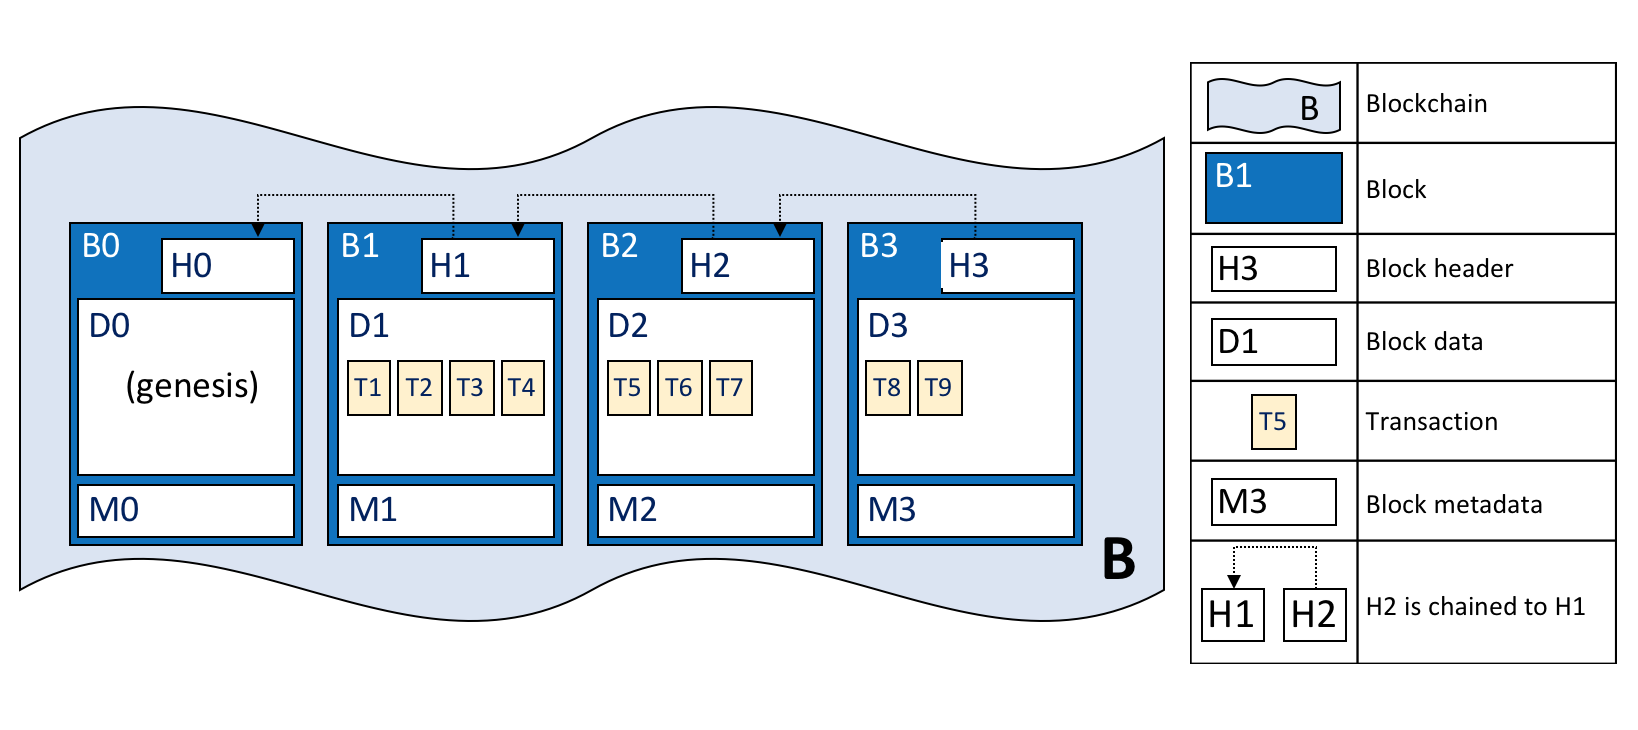
\includegraphics[scale=0.3]{recursos/blockchain-ledger.png}}
\caption{Estructura básica de una blockchain en Fabric.}
\label{blockchain}
\end{figure}
En la figura anterior, se puede observar como todos los bloques tienen tres partes, la cabecera, las transacciones y los metadatos. La cabecera es un hash formado por todas las transacciones del bloque, asi como la cabecera del bloque anterior. Esto genera una conexión inmutable entre todos los bloques, lo que da su nombre a la blockchain. En el cuerpo del bloque se encuentran las transacciones ordenadas por el \textit{orderer}, y en los metadatos se encuentra el certificado y la firma del creador del bloque para verificarlo en los nodos. Los metadatos tambien contienen un mapa de bits en el que se controla la validez de las transacciones del bloque.
Se puede observar también como el primer bloque no contiene ninguna transacción. Este es el bloque génesis, y solo contiene una transacción especial de configuración que define el estado inicial del \textit{channel}.
\subsection{Identidad y autenticación}
Al ser las redes Fabric privadas y permisionadas, los actores requieren de algún tipo de autenticación para poder acceder a ellas. Esto se gestiona mediante identidades digitales, que determinan los permisos y el acceso a la información de un actor determinado en una red. Estas identidades se encapsulan en certificados X.509.
\clearpage
\subsubsection{Organizaciones}
Una organización es un conjunto de actores que interactúa con un \textit{channel}, y la organización de cada actor esta determinada en su certificado digital, normalmente expedido por un autoridad de certificación. La asignación de organizaciones a cada actor en cada \textit{channel} la realiza el \acrshort{msp} de cada organización, junto al certificado de cada actor.
\begin{figure}[H]
\centerline{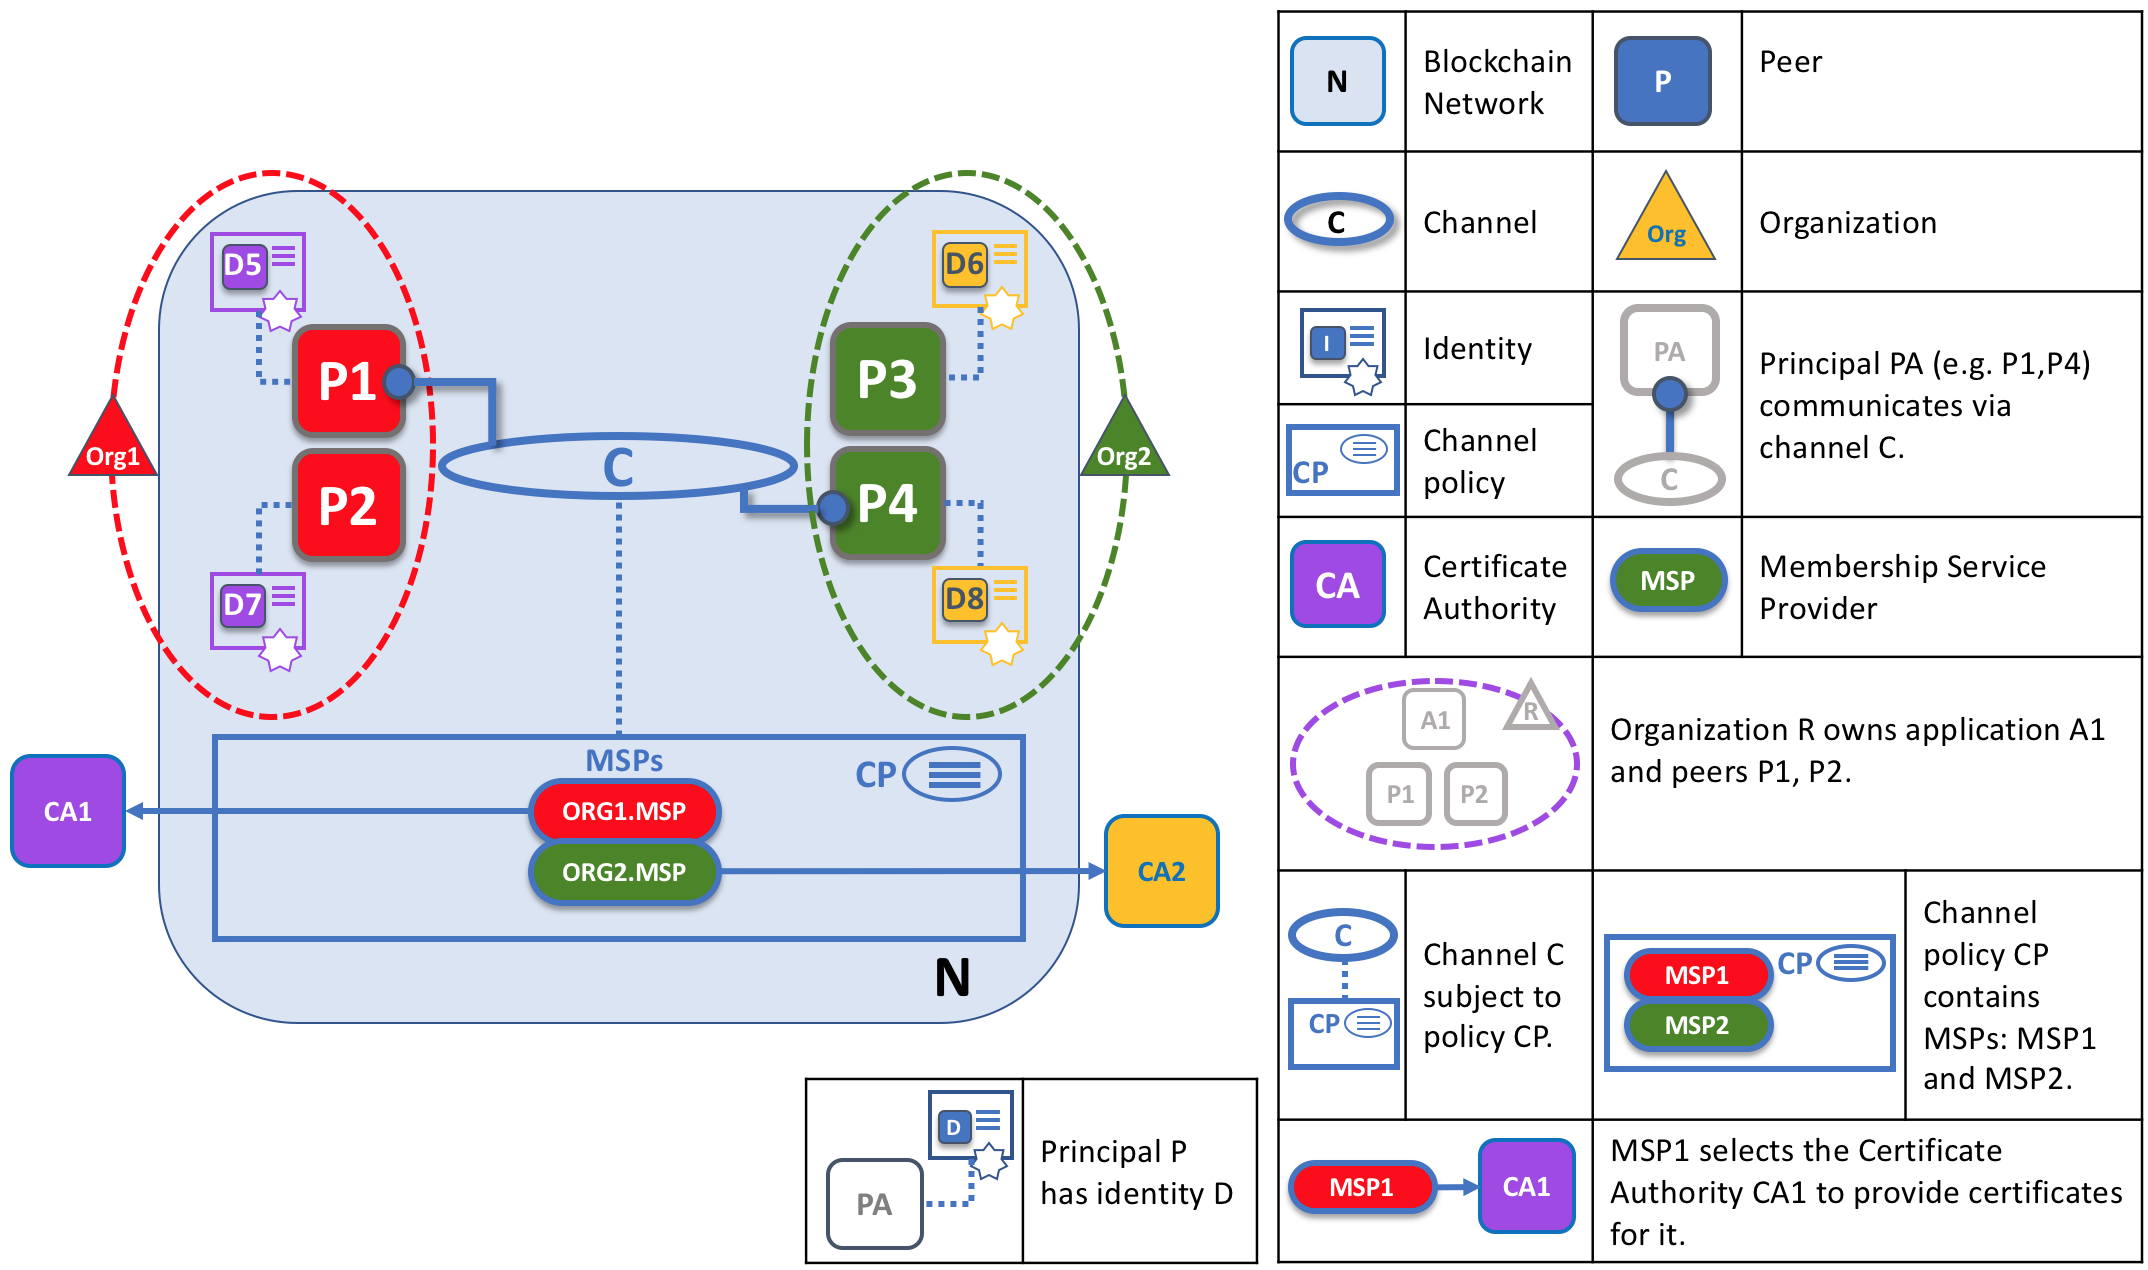
\includegraphics[scale=0.25]{recursos/orgs.png}}
\caption{Red Fabric con organizaciones y MSPs.}
\label{orgs-msp}
\end{figure}
En la figura anterior se puede observar como los \textit{peers} están dentro de organizaciones, con sus certificados correspondientes. La combinación del certificado y la identidad otorgada por el \acrshort{msp} da lugar a la identidad organizativa, denominada principal.
\subsubsection{Membership Service Providers}
Un \acrshort{msp} es el mecanismo utilizado para probar la identidad y la confianza en un actor dentro de una organización, además de otorgar roles a los participantes de la red.\\
Hay dos tipos de \acrshort{msp}s, locales y globales:
\begin{itemize}
    \item \textbf{MSP Local:} Los \acrshort{msp}s locales afectan a un nodo individualmente, y definen los permisos del mismo. Todos los nodos de la red deben tener definido un \acrshort{msp} local, ya que decide los derechos de participación a ese nivel.
    \item \textbf{MSP global:} Los \acrshort{msp}s globales controlan los derechos de participación a nivel de \textit{channel}. Todos los nodos del \textit{channel} pueden ver a los \acrshort{msp}s globales, y gracias a él pueden autenticar a todos los participantes del \textit{channel}. Todas las organizaciones que participen en un \textit{channel} deben tener un \acrshort{msp} propio, que decide que acciones pueden ejecutar los miembros en el \textit{channel}. A su vez, todos los \acrshort{msp}s de las organizaciones se incluyen en el \acrshort{msp} global.\\
    A diferencia de los \acrshort{msp}s locales, que se definen en el sistema de ficheros de cada nodo, los \acrshort{msp}s globales estan instanciados en todos los nodos del \textit{channel} y se sincronizan por consenso, de forma similar al \textit{ledger} del \textit{channel}.
\end{itemize}
\begin{figure}[H]
\centerline{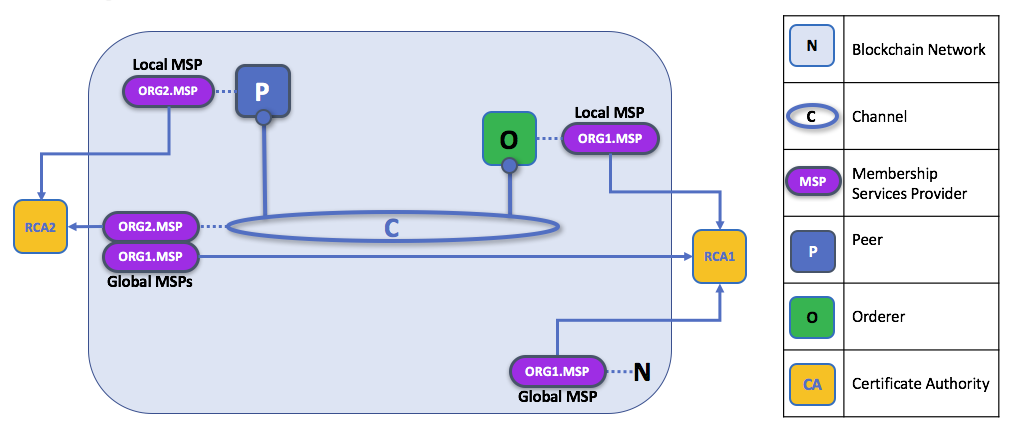
\includegraphics[scale=0.45]{recursos/msp.png}}
\caption{Red Fabric con MSPs locales y globales.}
\label{msps}
\end{figure}
En la imagen se puede observar una red típica, con un nodo de cada tipo y los \acrshort{msp} de cada organización. Estos se comunican tanto con los nodos en el canal como con las autoridades de certificación para asignar las identidades a cada miembro de la red.
\clearpage
\section{TrustOS}
Para concluir este capítulo, es interesante comentar la existencia de TrustOS, y su reciente relación con Alastria ID.
TrustOS es un conjunto de herramientas en forma de API desarrollada por Telefónica que simplifica la incorporación a una red blockchain de cualquier negocio o empresa, con diferentes módulos independientes para diferentes casos de uso, desplegados sobre redes ya existentes, y con la posibilidad de añadir APIs personalizadas o nuevos smart contracts dependiendo del caso de uso. Puede desplegarse sobre cualquier red de Hyperledger Fabric, y en el futuro también funcionará en redes Quorum y CORDA.
\begin{figure}[H]
\centerline{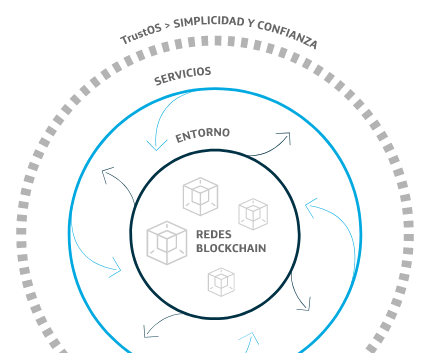
\includegraphics[scale=1]{recursos/trustos.png}}
\caption{TrustOS sobre servicios blockchain.}
\label{trustos}
\end{figure}
Funciona como una capa que encapsula los servicios blockchain, de forma que no es necesario poseer los conocimientos técnicos para incorporar funcionalidades blockchain a cualquier negocio. Se compone de cuatro módulos independientes, que disponen cada uno de un smart contract desplegado sobre varias redes blockchain, y una API para acceder comodamente a ellos. Los módulos son los siguientes:
\begin{itemize}
    \item \textbf{TRACK:} Se encarga de la representación digital de cualquier tipo de activo real, cuyo estado se monitoriza de forma transparente e inmutable, utilizando las características propias de la blockchain.
    \item \textbf{TOKEN:} Se encarga de crear ``tokens'', representaciones digitales de activos reales, dando valor real a cosas que por si solas no lo tendrían, creando la posibilidad de intercambios de activos entre empresas que confían mutuamente.
    \item \textbf{SETTLE:} Se encarga de proporcionar un sistema de consenso transparente y seguro entre los participantes, mediante el uso de smart contracts en la blockchain, para que no haya una entidad central administradora, y depositando la confianza en el propio proceso.
    \item \textbf{TRUST:} Esta relacionado con los demás módulos, y se encarga de registrar en una blockchain pública las operaciones de confianza entre miembros de la red, para crear un extra de transparencia a los procesos y garantizar la inmutabilidad de la información.
\end{itemize}
Recientemente, Inetum, un grupo empresarial estrechamente relacionado con Alastria, y Telefónica, han establecido un acuerdo para implementar el modelo Alastria ID sobre la plataforma de TrustOS, y desplegarlo en la red-H de Alastria.